\documentclass{beamer}
\usetheme{Madrid}

\usepackage{amsmath, amssymb, amsthm}
\usepackage{graphicx}
\usepackage{listings}
\usepackage{gensymb}
\usepackage{minted}
\usemintedstyle{friendly}
\definecolor{bg}{rgb}{0.95,0.95,0.95}
\usepackage[utf8]{inputenc}
\usepackage{hyperref}
\newcommand{\nCr}[2]{\,^{#1}C_{#2}}
\usepackage{gvv}\begin{document}

\title{11.16.3.8.5}
\author{EE24BTECH11012 \\ BHAVANISANKAR G S }
\date{\today}
\frame{\titlepage}

\begin{frame}
\frametitle{Question}
Three coins are tossed once. Find the probability of getting no head.\\
\end{frame}

\begin{frame}
\frametitle{Solution Outline}
\begin{enumerate}
	\item Define a random variable.
	\item Devise the PMF and CDF of the random variable.
	\item Deduce the required probability from the CDF expression.
\end{enumerate}
\end{frame}

\begin{frame}
\frametitle{Variables Used : }
\begin{center}
\begin{tabular}{|c|c|c|}
\hline 
\textbf{Variable name} & \textbf{Description} \\
\hline 
$\vec{S}$ & Sample space \\
\hline 
$\vec{X}$ & Random variable corresponding to the number of heads \\
\hline
$p$ & Toss corresponding to head \\
\hline
$F_{\vec{X}} (x)$ & Cumulative distribution function ( CDF ) \\
\hline
$p_{\vec{X}} (x)$ & Probability Mass function ( PMF ) \\
\hline
\end{tabular}
\end{center}
\end{frame}

\begin{frame}
	Let us assume the random variable to be the sum of three Bernoulli Random Variables.
\begin{align}
	\vec{X} &= \vec{X_{1}} + \vec{X_{2}} + \vec{X_{3}} \\
	\vec{X_{i}} &= 
	\begin{cases}
		1 & , \text{ Outcome - head } \\
		0 & , \text{ Outcome - tail }
	\end{cases} \\
	\implies p_{X_{i}} (k) &= 
	\begin{cases}
		1 - p & , k = 0 \\
		p & , k = 1
	\end{cases}
\end{align}
Considering all the outcomes as equally likely, we have
\begin{align}
	p &= \frac{1}{2} \label{eq:p}
\end{align}
\end{frame}

\begin{frame}
\frametitle{Solution}
For the given question, let $\vec{X}$ denote the number of heads. The sample space corresponding to the given scenario is tabulated below. \\
\begin{center}
\begin{tabular}{|c|c|c|}
\hline 
\textbf{Event} & \textbf{Sample space} \\
\hline
$p_{\vec{X}} (0)$ & \cbrak{TTT} \\
\hline
$p_{\vec{X}} (1)$ & \cbrak{TTH, THT, HTT} \\
\hline
$p_{\vec{X}} (2)$ & \cbrak{HHT, HTH, THH} \\
\hline
$p_{\vec{X}} (3)$ & \cbrak{HHH} \\
\hline
\end{tabular}
\end{center}


\end{frame}

\begin{frame}
By the properties of Z-transform of \textbf{Probability Mass Function}, we have
\begin{align}
	M_{\vec{X}} (z) &= M_{\vec{X_{1}}} (z) M_{\vec{X_{2}}} (z) M_{\vec{X_{3}}} (z) \\
	M_{\vec{X_{1}}} &= \sum_{n = - \infty}^{\infty} p_{\vec{X_{1}}} (n) z^{-n} = (1 - p) + \brak{p}z^{-1} \\
	M_{\vec{X_{2}}} &= \sum_{n = - \infty}^{\infty} p_{\vec{X_{2}}} (n) z^{-n} = (1 - p) + \brak{p}z^{-1} \\
	M_{\vec{X_{3}}} &= \sum_{n = - \infty}^{\infty} p_{\vec{X_{3}}} (n) z^{-n} = (1 - p) + \brak{p}z^{-1} \\
	M_{\vec{X}} (z) &= \brak{(1 - p) + \brak{p}z^{-1}}^3 \\
	                &= \sum_{k = -\infty}^{\infty} \nCr{3}{k} \brak{1-p}^{3-k} p^{k} z^{-k} \\
	p_{\vec{X}} (k) &= \nCr{3}{k} \brak{1-p}^{3-k} p^{k} \label{eq:pm}
\end{align}

\end{frame}

\begin{frame}
Substituting \eqref{eq:p} in \eqref{eq:pm}, we have
\begin{align}
	p_{\vec{X}} (k) &= \frac{\nCr{3}{k}}{8} \label{eq:pmf}
\end{align}
The PMF is then given by - 
\begin{align}
p_{\vec{X}} (k) &= 
\begin{cases}
	\frac{\nCr{3}{k}}{8} & 0 \leq k \leq 3, k \in \mathbb{W} \\
	0 & otherwise
\end{cases} \\
\implies p_{\vec{X}} (k) &= 
\begin{cases}
	\frac{1}{8} & k = 0 \text{ or }  k = 3\\
	\frac{3}{8} & k = 1 \text{ or } k = 2\\
	0 & \text{ otherwise }
\end{cases}
\end{align}
\end{frame}

\begin{frame}
\frametitle{CDF}
The corresponding \textbf{Cumulative Distribution Function} can then be written as - 
\begin{align}
  F_{X}\brak{k} &= \sum_{i = -\infty}^k\comb{3}{i}\brak{\frac{1}{2}}^3 \\
  &= \begin{cases}
    0 & k < 0\\
    \comb{3}{0}\brak{\frac{1}{2}}^3 & 0 \le k < 1\\
    \comb{3}{1}\brak{\frac{1}{2}}^3 + \comb{3}{0}\brak{\frac{1}{2}}^3 & 1 \le k < 2\\
    \comb{3}{2}\brak{\frac{1}{2}}^3 + \comb{3}{1}\brak{\frac{1}{2}}^3 + \comb{3}{0}\brak{\frac{1}{2}}^3  & 2 \le k < 3\\
    \comb{3}{3}\brak{\frac{1}{2}}^3 + \comb{3}{2}\brak{\frac{1}{2}}^3 + \comb{3}{1}\brak{\frac{1}{2}}^3 + \comb{3}{0}\brak{\frac{1}{2}}^3 & k \geq 3\\
  \end{cases}
\end{align}
\end{frame}

\begin{frame}
\begin{align}
\implies F_{\vec{X}}(k) = Pr(\vec{X} \leq k) =
\begin{cases}
    0 & k < 0 \\
    \frac{1}{8} & 0 \leq k < 1 \\
    \frac{1}{2} & 1 \leq k < 2 \\
    \frac{7}{8} & 2 \leq k < 3 \\
    1 & k \geq 3
\end{cases}
\end{align}
\begin{align}
	F_{\vec{X}} \brak{0} &= P \brak{ \vec{X} <= 0 } \\
	                     &= \frac{1}{8}
\end{align}
\end{frame}

\begin{frame}
\frametitle{Simulation}
\begin{enumerate}
	\item Generate a random number using the \textbf{rand()} function. 
	\item Restrict the random number to either $0$ or $1$ by using rand() \% 2 operator, and assign it to head ( H ) and tail ( T ).
	\item Count the number of favourable outcomes by iterating for a large number of trials.
	\item Divide it by the total number of trials to get the desired PMF.
	\item CDF can then be simulated by summing the required PMFs.
\end{enumerate}
\end{frame}

\begin{frame}
\frametitle{PMF - Plot}
\begin{figure}[h]
\centering
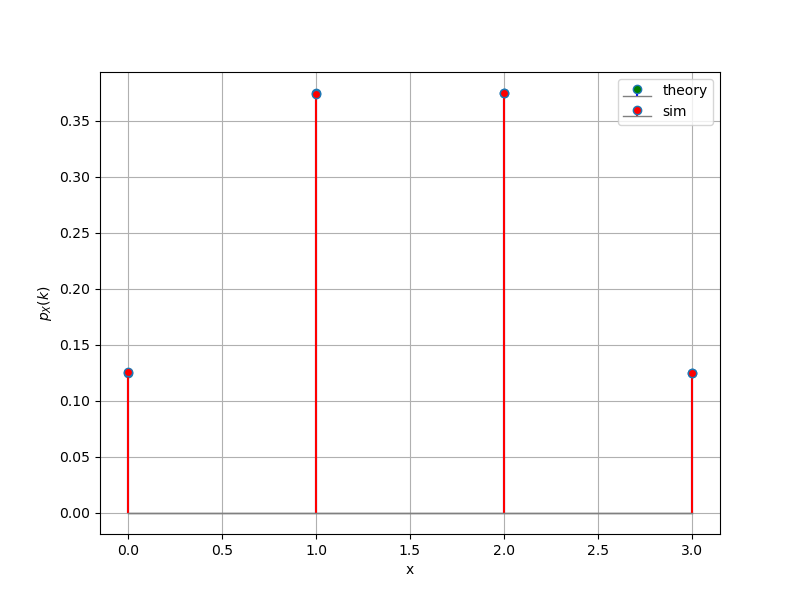
\includegraphics[width=\columnwidth]{figs/pmf.png}
\caption{Probability Mass Function}
\label{fig:Plot1} 
\end{figure}
\end{frame}

\begin{frame}
\frametitle{CDF - Plot}
\begin{figure}[h]
\centering
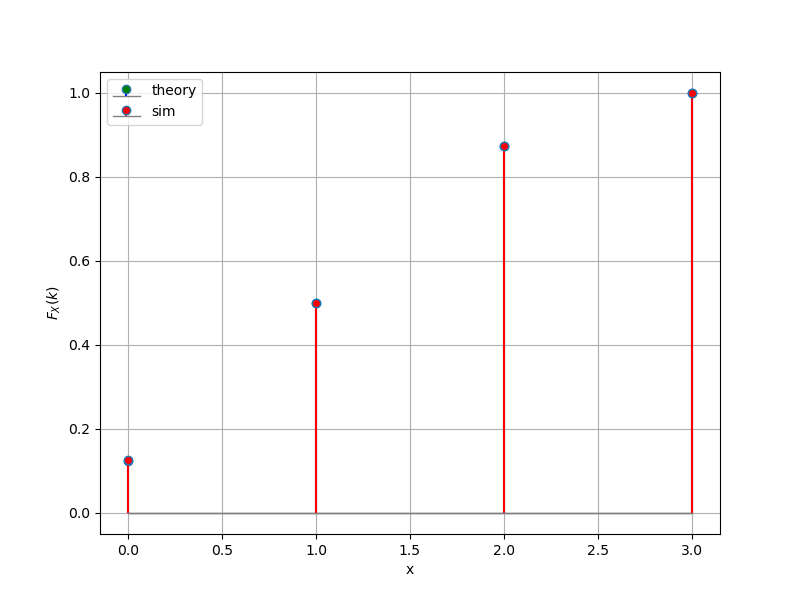
\includegraphics[width=\columnwidth]{figs/cdf.png}
\caption{Cumulative Distribution Function}
\label{fig:Plot2} 
\end{figure}
\end{frame}
\end{document}
